
\documentclass[]{article}

\title{Ajuste de curvas }

\date{}
\usepackage{braket}
\usepackage{bbold}
\usepackage{amsmath,amsfonts,amssymb,amsthm,booktabs}
\usepackage[margin=1.0in]{geometry}
\usepackage{graphicx}
\usepackage{chngcntr}
\usepackage{floatrow}
\usepackage{chngcntr}
\usepackage{hyperref}
\usepackage[spanish]{babel}
\usepackage[svgnames]{xcolor}

\usepackage{floatrow}
\floatsetup[table]{capposition=top}

\renewcommand{\spanishtablename}{Cuadro}
\usepackage{listings}
\usepackage[%
    font={small,sf},
    labelfont=bf,
    format=hang,    
    format=plain,
    margin=0pt,
    width=0.8\textwidth,
]{caption}
\usepackage[list=true]{subcaption}
\lstset{language=R,
    basicstyle=\small\ttfamily,
    stringstyle=\color{DarkGreen},
    otherkeywords={0,1,2,3,4,5,6,7,8,9},
    morekeywords={TRUE,FALSE},
    deletekeywords={data,frame,length,as,character},
    keywordstyle=\color{blue},
    commentstyle=\color{DarkGreen},
}

\counterwithin{figure}{section}
\renewcommand*{\figureautorefname}{Figura}


\usepackage[backend=biber]{biblatex}
\addbibresource{ref.bib}

\begin{document}
	\maketitle
	\begin{center}


\centerline{\textbf{TAREA 7} } 
\textbf{ }

\centerline{Alumno: } 
\centerline{Joaquín Arturo Velarde Moreno}


	\end{center}
	

\section{Introducción}
El objetivo del siguiente reporte es describir cómo se obtiene la correlación lineal a través de varios ejemplos de funciones matemáticas; ver su representación gráfica y la forma de su curva. Para cumplir con este objetivo, usaremos el programa R 4.0.2 \cite{rproject} y de este modo, haremos cálculos con una serie de datos.
Usaremos como apoyo el material de la Dra. Elisa Schaefer \cite{MaterialClase}.


\section{Definición correlación lineal}
La correlación es una medida de la presencia de una relación lineal en un conjunto de datos que provienen de dos variables medidas al mismo tiempo sobre cada individuo; también se les conoce como datos bivariados.
Estos se pueden representar gráficamente, como se muestra en una encuesta que se hizo a alumnas de una escuela (\autoref{fig:CorrelacionTest}). En la que se midió el peso y la altura de cada una de ellas; en la representación gráfica se puede ver que hay una relación entre el peso y estatura de estos individuos.

\begin{figure}[hbt!] 
\centering 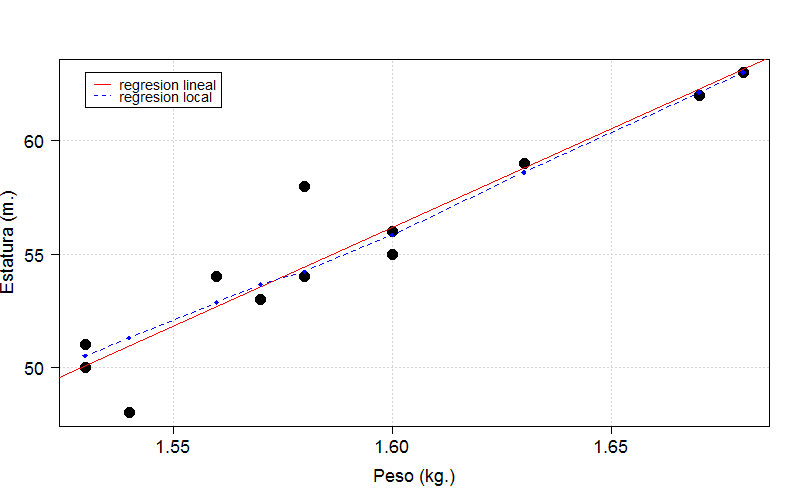
\includegraphics[width=.7\linewidth]{Figuras/CorrelacionTest.png}                 \caption{Relación entre peso(kg.) y altura(m.) de alumnas.}
\label{fig:CorrelacionTest}
\end{figure}


En el presente reporte usaremos la correlación de Pearson, al cual denotaremos por \textit{r}, el rango de la correlación \textit{r} va de \textit{1} a \textit{-1}, esto puede generar 3 casos (\autoref{fig:casos}).

\begin{itemize}
	\item $r$ igual a $1$: positiva.
	\item $r$ igual a $-1$: negativa.
	\item $r$ igual a $0$:  sin correlación.

\end{itemize}




La mayoría de las veces no tendremos mediciones exactas para cada caso, si no que tendremos un aproximado a cada estado, con este aproximado podremos decidir si nuestros datos tienen una relación o si son independientes entre si.

\begin{figure}[hbt!]
\centering
\subcaptionbox{Correlación negativa $Y$ disminuye cuando $X$ crece.}{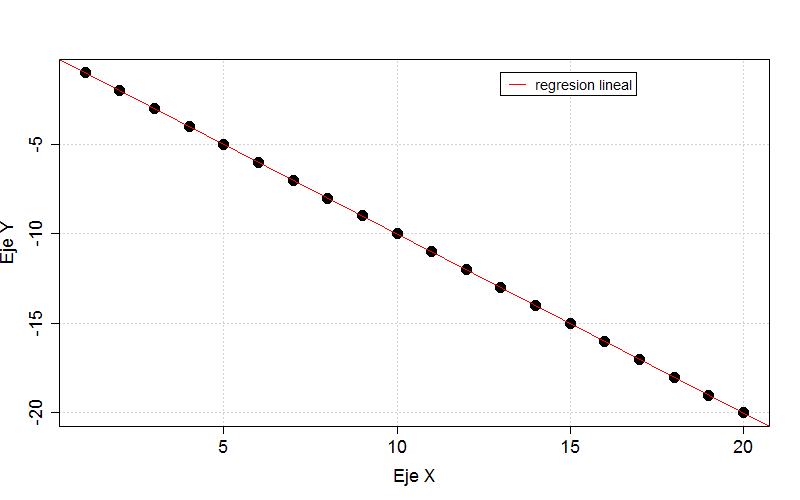
\includegraphics[width=0.3\textwidth]{Figuras/CorrelacionNegativa.png}}%
\hfill
\subcaptionbox{No hay relación alguna en los datos.}{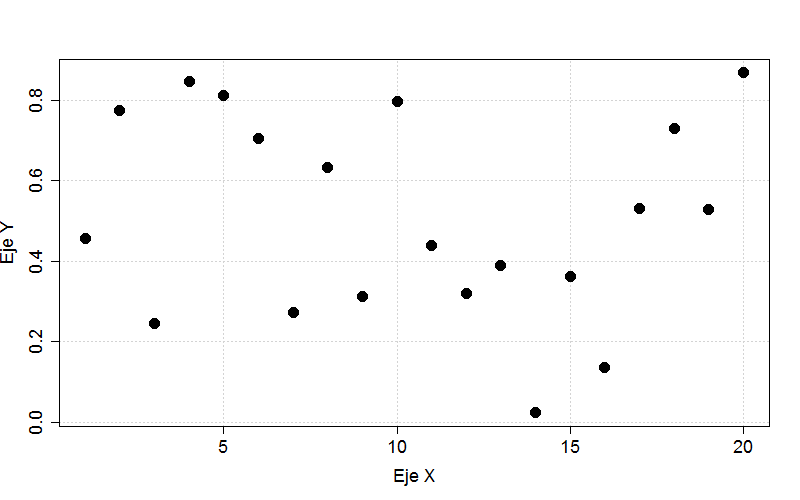
\includegraphics[width=0.3\textwidth]{Figuras/SinCorrelacion.png}}%
\hfill
\subcaptionbox{Correlación negativa $Y$ aumenta cuando $X$ crece.}{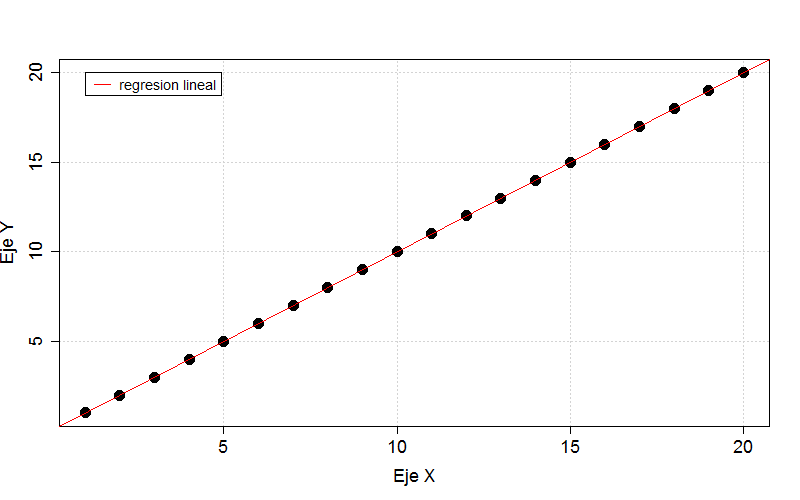
\includegraphics[width=0.3\textwidth]{Figuras/CorrelacionPositiva.png}}%
\hfill
\caption{Correlaciones en sus valores negativo, positivo y 0.}
\label{fig:casos}
\end{figure}

\section{Fórmula}
La correlación de Pearson puede ser obtenida por la siguiente expresión:
\[\ \frac{\Sigma\left(x\ \times\ y\right)\ -\ \frac{1}{n}\left(\Sigma x\ \times\Sigma y\right)}{\sqrt{\left(\Sigma x^2-\frac{1}{2}\left(\Sigma x\right)^2\right)\times\left(\Sigma y^2-\frac{1}{2}\left(\Sigma y\right)^2\right)}}.\]

donde:
\begin{itemize}
	\item $x\ y\ y$ son nuestros datos bivariados.
	\item $n$ es el numero de datos.
\end{itemize}
Esta ecuación puede ser expresada en R de la siguiente manera:
  \begin{lstlisting}

    n                  <- length(VectorX)
    SumatoriaX         <- sum(VectorX)
    SumatoriaY         <- sum(VectorY)
    
    numerador          <- sum(VectorX * VectorY) - (SumatoriaX * SumatoriaY) / n
    denominadorX       <- sum(VectorX **2) - (SumatoriaX**2) / n
    denominadorY       <- sum(VectorY **2) - (SumatoriaY**2) / n
    denominador        <- sqrt(denominadorX * denominadorY)
    correlacion        <- numerador / denominador
   \end{lstlisting}
Existe una manera mas sencilla de hacer este calculo, obteniendo los promedios de cada vector  a los cuales denotaremos como $X\ y\ Y$, pudiéndose expresar de la siguiente manera:
\[\ \frac{\Sigma\left(x\ \times\ y\right)}{\sqrt{\Sigma x^2\times\Sigma y^2}}.\]
donde:
\begin{itemize}
	\item $y$ = $Y - \mu Y$.
	\item $x$ = $X - \mu X$.

\end{itemize}
Esta ecuación puede ser expresada en R de la siguiente manera:
  \begin{lstlisting}
    x        <- VectorX - mean(VectorX)
    y        <- VectorY - mean(VectorY)
    
    correlacion     <- sum(x * y) / sqrt(sum(x**2) * sum(y**2))
   \end{lstlisting}

\section{Transformadas}
No todos los conjuntos de datos vienen de manera lineal, algunas vienen muy dispersos y otros forman curvas, como es el caso del ejemplo de la función $f\left(x\right)\ =\ x^2$ (\autoref{fig:Curva}). 
En estos casos lo mejor es trabajar con transformadas, estas son manipulaciones que se hacen a un vector de los datos para poder acomodarlos una relación lineal. 
una opción sencilla es la escalera de Tukey:

\begin{table}[hbt!]
\begin{center}
 \begin{tabular}{c|r|r|r|r|r|r|r}
    $\lambda$ & $-2$ & $-1$ & $\frac{1}{2}$ & $0$ & $\frac{1}{2}$ & $1$ & $2$\\
   \hline
    & $\frac{1}{x^2}$ & $\frac{1}{x}$ & $\frac{1}{\sqrt{x}}$ & $\log x$ & $\sqrt{x}$ & $x$ & $x^2$ \\
   \hline
 \end{tabular}
 \caption{Escalera de Tuker con un rango de -2 a 2.}
 
\label{t1}
\end{center}
\end{table}

Podemos calcular comparar cada transformada en R de la siguiente manera:
  \begin{lstlisting}
      for(i in seq(-2,2,1))
      {
          if(i > 0)
          { z <- x^i}
          else if(i < 0)
          { z <- -1*x^i}
          else
          { z <- log(x)}
          cor(y,z)
       }
   \end{lstlisting}

Dada la función $f\left(x\right)\ =\ 3x^2$ podemos buscar una transformada por la escalera de Tukey que nos encuentre el $\lambda$ que mas haga una relación lineal en nuestros conjuntos.



\begin{figure}[hbt!]
\centering
\subcaptionbox{Curva de la función $f\left(x\right)\ =\ 3x^2$.}{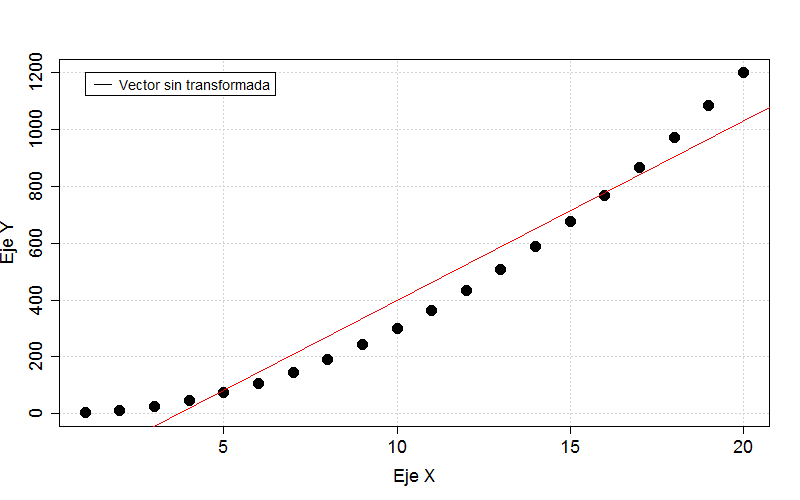
\includegraphics[width=0.3\textwidth]{Figuras/SinTransformada.png}}%
\hfill
\subcaptionbox{Transformada con $\lambda = -2$.}{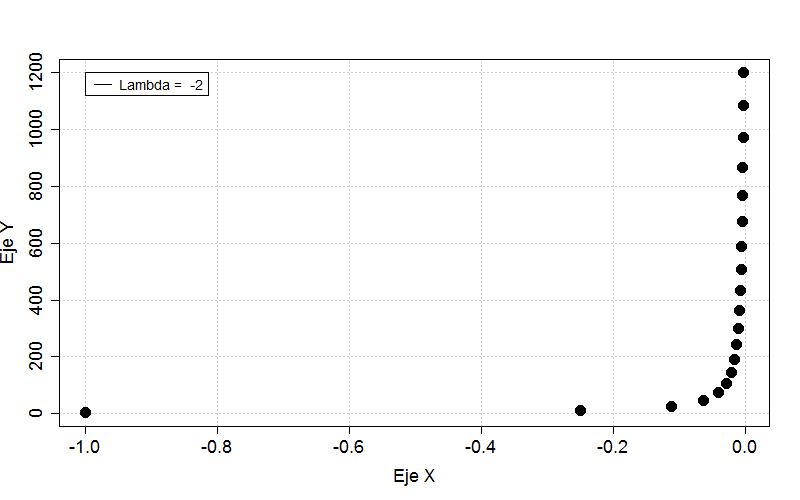
\includegraphics[width=0.3\textwidth]{Figuras/Lambda-2.png}}%
\hfill
\subcaptionbox{Transformada con $\lambda = -1$.}{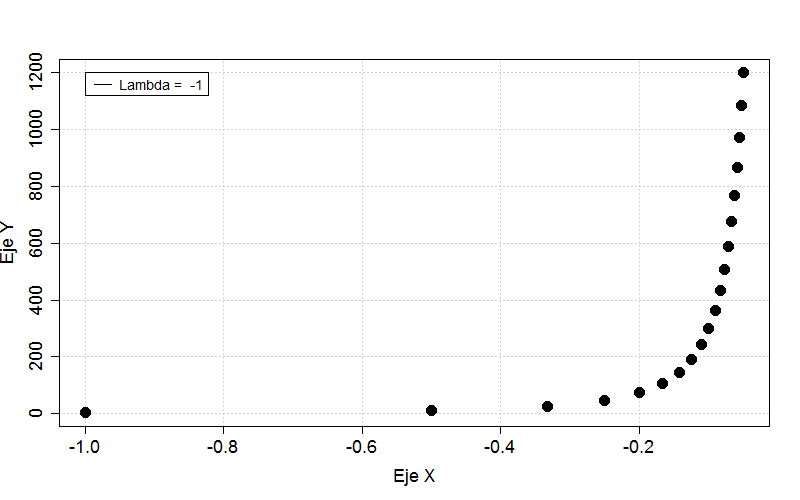
\includegraphics[width=0.3\textwidth]{Figuras/Lambda-1.png}}%
\hfill
\subcaptionbox{Transformada con $\lambda = 0$.}{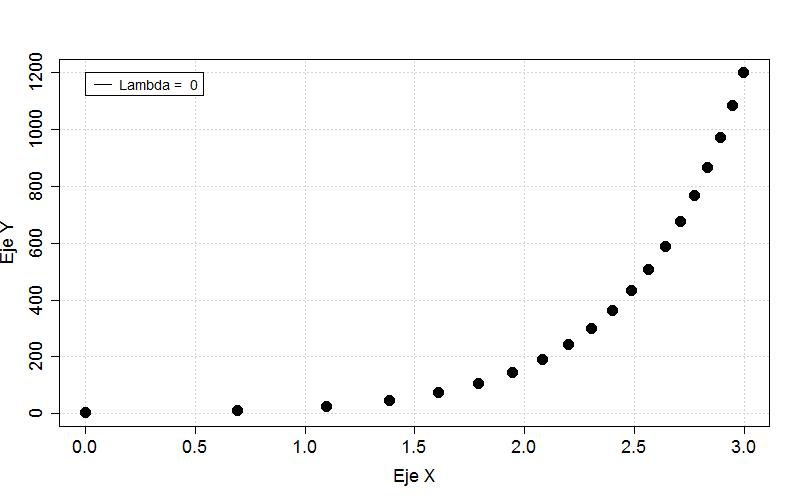
\includegraphics[width=0.3\textwidth]{Figuras/Lambda0.png}}%
\hfill
\subcaptionbox{Transformada con $\lambda = 1$.}{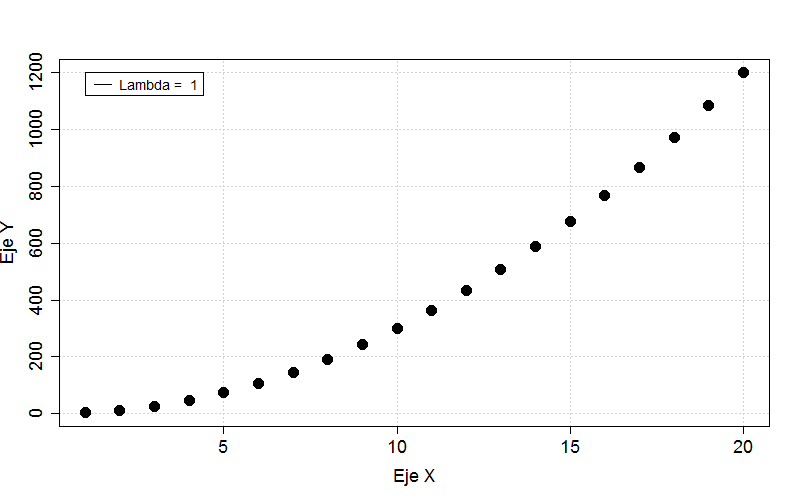
\includegraphics[width=0.3\textwidth]{Figuras/Lambda1.png}}%
\hfill
\subcaptionbox{Transformada con $\lambda = 2$.}{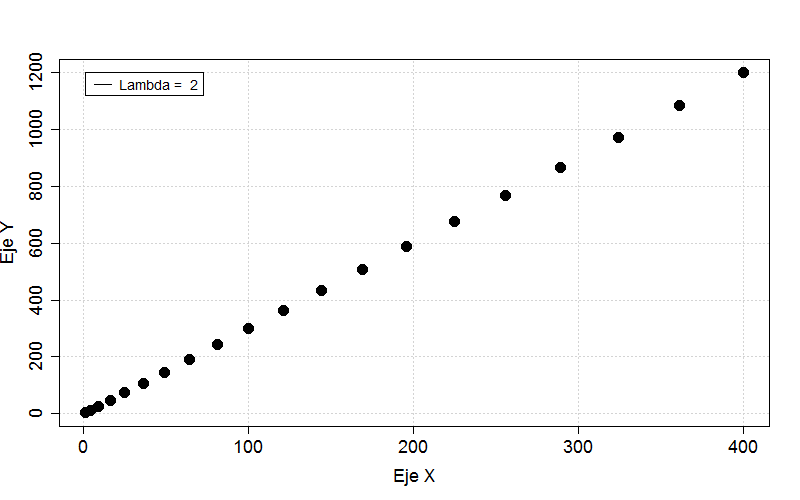
\includegraphics[width=0.3\textwidth]{Figuras/Lambda2.png}}%
\hfill
\caption{Transformadas de la función $f\left(x\right)\ =\ 3x^2$.}

\label{fig:casos}
\end{figure}


Una alternativa optimizada es la transformada Box-Scott, en esta expresion $X$ se transforma a $\frac{(x^{\Lambda }\ -\ 1)}{\Lambda }$.
Podemos calcular comparar cada transformada en R de la siguiente manera:
  \begin{lstlisting}
      for(i in seq(-2,2,0.05))
      {
          z <- (abs(x)^i-1)/i
          w <- c(w,cor(y,z))
          v <- c(v,i)
      }
      plot(v, w)
   \end{lstlisting}

\begin{figure}[hbt!] 
\centering 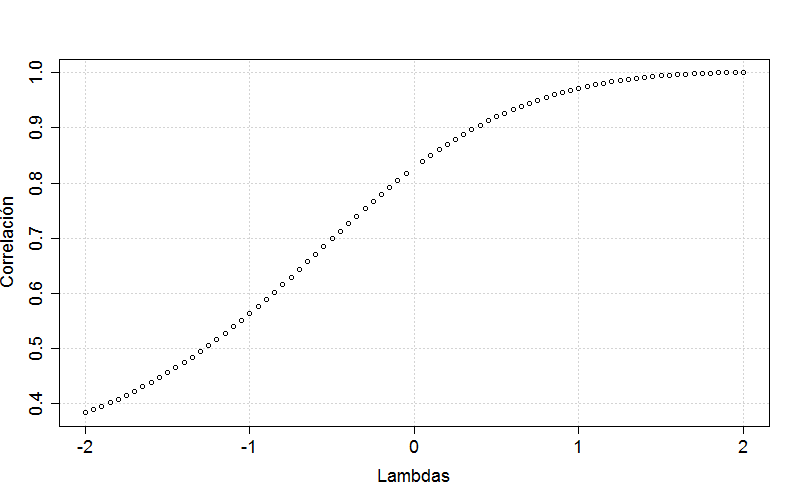
\includegraphics[width=.7\linewidth]{Figuras/box-cox.png}                 \caption{Lambdas y su correlación usando la transformada de Box-Scott en la función $f\left(x\right)\ =\ 3x^2$.}
\label{fig:Correlacionbox}
\end{figure}

\begin{figure}[bt!]
\centering 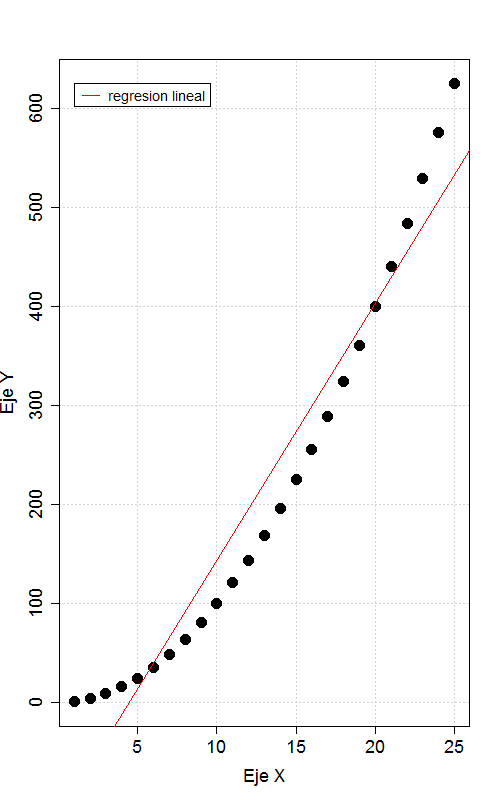
\includegraphics[width=.7\linewidth]{Figuras/CorrelacionCurva.png}                 \caption{Relación entre el conjunto X y el Y al aplicar $f\left(x\right)\ =\ x^2$.}
\label{fig:Curva}
\end{figure}




\printbibliography[title={Referencias}]
\end{document}
